\documentclass[11pt]{article}
\usepackage[utf8]{inputenc}
\usepackage{amsmath,amssymb,hyperref,array,xcolor,multicol,verbatim,mathpazo}
\usepackage[normalem]{ulem}
\usepackage[pdftex]{graphicx}
\usepackage{fullpage}
\usepackage{import}
\usepackage{adjustbox}
\usepackage{booktabs}
\usepackage[font=footnotesize,labelfont=bf]{caption}
%\captionsetup{justification=raggedright,singlelinecheck=false}


\usepackage[backend=biber,style=authoryear,
sorting=ynt,citestyle=authoryear]{biblatex}
\addbibresource{papercitations.bib}
\usepackage{setspace}
%\singlespacing
\doublespacing
\addtolength{\skip\footins}{2pc plus 5pt}

\title{Labor Markets and Technological Change: Evidence from Electronic Health Records}
\author{Hanna Glenn}
%\date{\today}

\DeclareLabeldate[online]{%
  \field{date}
  \field{year}
  \field{eventdate}
  \field{origdate}
  \field{urldate}
}

\begin{document}

\maketitle



\vspace{1.5cm}

The interaction between technological innovation and labor markets has a direct impact across industries; job characteristics such as displacement, creation, and satisfaction are all prevalent for many workers (\cite{autor2003skill}, \cite{fallick1996review}, \cite{akerlof1988job}). Labor market changes for one job type may have rippling effects on populations serviced by that industry. It is straightforward to see this for a physician since choices and labor markets directly affect patient accessibility and quality of care received. For example, physician burnout is correlated with lower patient satisfaction (\cite{shanafelt2002burnout}), physician shortages are linked to higher mortality rates (\cite{gong2019higher}), and administrative regulations on physicians such as standardized checklists may be associated with lower mortality in surgical settings (\cite{treadwell2014surgical}). Physician labor markets are an important topic of study because of their implications on care. I investigate physician labor market changes as a result of a major technology change in the U.S. healthcare system, the implementation of electronic health care record systems, which have been emphasized as a cause of burnout and may induce changes to physician labor market decisions.

Electronic Health Records (EHRs) are computerized medical records which include detailed accounts and notes of medical history, stored in advanced systems with additional capabilities such as providing suggestions for care. EHRs have have become increasingly relevant in the U.S. since 2008, in part after former President Obama stated in 2009, “To improve the quality of our health care while lowering its cost, we will make the immediate investments necessary to ensure that, within five years, all of America’s medical records are computerized.” (\cite{presquote}). The movement towards digitization in health care was expected to have immediate and substantial impacts on efficiency. A 2005 study estimated hundreds of billions of dollars saved if health information technology were to be fully implemented (\cite{hillestad2005}). Such expectations led the U.S. government to incentivize the use of EHRs in hospitals with the the Health Information Technology for Economic and Clinical Health (HITECH) Act in 2008 (\cite{hitech})\footnote{This legislation subsidized hospitals which used EHRs “meaningfully”According to Quatris Healthco, meaningful use standards proceeded in three stages over time. In Stage 1 (2010), MU focused on data capturing and sharing. In Stage 2, which began in late 2012, MU extended to using EHRs for patient incorporation and using the technology as a helper in care. Stage 3 went from 2014-2016 and focused on making data accessible across hospitals (\cite{meanuse})}. The percentage of hospitals with the capability of using a basic EHR system went from 9 percent in 2008 to 84 percent in 2015 (\cite{stats}), revealing the nationwide movement towards digitization.

Physicians, as primary users of this technology, play a meaningful role in whether potential benefits of EHRs are realized. With the rapid implementation of a complex technology, the practical tasks that take place in a physician's daily life changed just as rapidly. In interviews, physicians reported that when using EHRs they are less satisfied with their job and have higher stress levels. Senior physicians in particular were found to “loathe the cumbersome, time-consuming data entry that comes with using EHRs.” (\cite{CollierBurnout}). The frustration of using a new technology raises the cost of working in specific hospitals, which may lead physicians on the margin to make changes in labor market choices such as exiting the labor market altogether. Further, the short and long run impacts of EHRs on physician productivity could vary greatly due to the immediate learning curve that subsides over time.  Treating EHR implementation in hospitals as exogenous to an individual physician, I use difference in difference with heterogeneous treatment timing to understand the effect of EHR implementation in hospitals on physician labor market outcomes: retirement, choice of work setting, and amount of patients seen.

Using CMS Shared Patient data and Medicare Data on Provider Practice and Specialty (MD-PPAS), I construct a physician-level panel from 2009-2017 consisting of hospitalists and other general practice physicians connected to hospitals. The data captures the extent to which the physician in exposed to EHRs in various hospitals, several labor market outcomes, and demographic information such as zip code, age, and gender. I analyze the impact of EHR exposure on the following physician decisions: (1) retirement, (2) where to physically work (changing hospitals or moving to office based settings), and (3) the number of patients seen by the physician. Common to each specification is the use of treatment variables capturing a physicians' level of EHR exposure in hospitals on two dimensions: working in any hospital that implements an EHR, and working in a low-integrated hospital that implements an EHR. A key assumption that underlies the analysis is that EHR exposure is exogenous to physicians. While this assumption is reasonable in many settings, there may be instances where a physician is involved in hospital decisions. This is the reason I include a second definition of EHR exposure that only considers hospitals where vertical integration between physicians and the hospital are low, as this indicates a much lower probability that EHR implementation is endogenous. In the Appendix I consider different thresholds of exposure as treatment variables for robustness. 

Retirement typically takes place late in life, which is no different for physicians. The average physician retirement age is 65 (\cite{collier2017challenges}) However, the data reveals that even physicians as young as 35 are "retiring". Young physicians are likely not retiring in the formal sense, but leaving a clinical setting for a more administrative setting. Alternative careers include teaching, consulting, or medical malpractice expert. My data does not allow granular details of what physicians do when they drop out of clinical settings, so I define retirement vaguely as the decision to cease clinical work altogether. The implications of physicians retiring are the same whether they are young or old, that access to care issues may have been exemplified. Contrary to previous work stating that physicians do not retire based on work environment (\cite{Bahrami2002}), I find that EHR implementation led to a .1 ppt increase in the likelihood of a senior physician retiring. While there were occurrences of young physicians leaving clinical work, there is no evidence that it was because of EHR implementation.

Not everyone chooses to forego clinical work altogether. However, there may be margin to change physical place of work if physicians are not satisfied with their experience at a given hospital, whether it is because of burnout, loss of autonomy, or factors unrelated to EHRs. I investigate whether physicians switch from primarily hospital based work to smaller office based settings, or switch hospital locations? To answer this question, I limit the sample to any physicians who did not retire and use the same event study framework to estimate the effect of EHR implementation on whether the physician switches zip codes or increases office-based patients. I find that \textcolor{red}{put exact findings here and their implications (are physicians trying to shift away from an autonomous standard of care they have to abide by?)}. 

Finally, I investigate the effect of the technology implementation on productivity within hospitals, measured by the number of patients seen. 


\textcolor{red}{Add a paragraph discussing sensitivity analysis or mechanisms.}

This paper's contribution to the space is threefold: (1) this is the first study to my knowledge that empirically analyzes the relationship between physician labor markets and EHRs, (2) since there seems to be a disconnect between the potentials of EHR technologies and the realized effects, this paper will speak to a potential mechanism that is causing this puzzle, and (3) this study covers the time period of the major EHR boom in healthcare, whereas most studies mentioned above utilize data before 2010. \textcolor{red}{This needs to be expounded upon a lot. Perhaps one or two paragraphs for each area of contribution.}

The effects of EHR implementation on costs and quality of healthcare prior to 2010 have been studied extensively. Despite many case studies and hospital-level analysis that indicate a large decrease in mortality rates (\cite{Buntin2011TheResults}), more recent economic research has showed that the technology has only improved health outcomes for patients with severe conditions, but have not led to improvements for the median patient (\cite{Agha2014TheCare}; \cite{McCullough2016HealthCoordination}; \cite{Meyerhoefer}). Further, there have been no significant cost decreases due to EHRs in the short or long run. If any cost reductions are realized at all, they are at least 6 years after implementation (\cite{dranove2014trillion}). As discussed earlier, these findings are puzzling due to the expected benefits of EHRs. This paper contributes to our knowledge of this area in re-framing past finding into a patient access to care problem instead of an efficiency problem.

\textcolor{red}{Expand both contribution and literature review and combine them to flow better.}


\newpage


\section{Institution}

EHRs have been an important feature of healthcare since the 1980s and 1990s. Early in its existence, the technology was mainly produced and used by academic medical centers whose primary goal was to create efficiency in billing and/or scheduling. Prior to computerization, physicians were not able to interface directly with EHRs, and thus were not drastically affected by their implementation. The cost of utilizing an EHR was large and increasing in the amount of capabilities of the system, which led to the widespread view that EHRs were strictly complements to paper records, not a feasible substitute. As computers were made more portable, the usability of EHRs increased, creating what is known as the "physician workspace": a computer station for a physician to interface directly with an EHR to record patient updates. Despite usability, physicians kept the view that EHRs were purely complementary to paper due to burdensome data entry. Automation in data entry was non-existent, making it extremely time consuming for the user. Even when automation was developed for particular machines that performed monitoring, the hospital still held responsibility for the accuracy of information and therefore required physicians to manually check each data entry. 

The HITECH Act was passed in 2009, setting aside government funds to subsidize hospitals who used EHRs according to certain guidelines. The guidelines include having at least 80\% of patients in the system, regularly recording answers to specific questions, and protecting the security of the system to ensure privacy. Immediately, EHR companies took advantage of the legislation and began marketing campaigns centered around their system being eligible to earn the hospital subsidies. Hospitals began receiving payments for the first stage of meaningful use in 2011. This resulted in a 75 percentage point increase in the number of hospitals with EHRs from 2009 to 2015 (\cite{stats}). Figure \ref{fig:meanuse} shows a comparison of U.S. hospitals who have received stage 1 of the meaningful use subsidy in 2011 vs. 2013. 

\vspace{3mm}
\begin{figure}[ht]
    \centering
    \caption{Hospitals Receiving Meaningful Use Stage 1 Subsidy}
    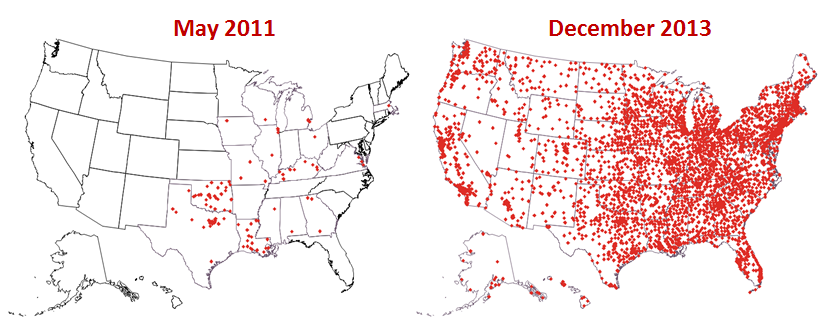
\includegraphics[scale=.6]{Objects/QS-Hospitals-Receiving-Payments-for-MU-and-Adoption.png}
    \caption*{Source: HealthIT.gov}
    \label{fig:meanuse}
\end{figure}
\vspace{3mm}

While EHRs were widely utilized in hospitals by 2015, physicians still continue to report frustration. For every patient seen, a primary care physician spends an average of 16 minutes actively using an EHR, an amount of time that often exceeds face to face time with the patient (\cite{overhage2020physician}). The tasks that may take place during this time include viewing or inputting patient information, ordering services such as tests or prescriptions, navigating the system, or communication. Appendix (\textcolor{red}{section}) includes a computer screen image of what a physician may see when looking at EHRs. Because of the added administrative burden, "some healthcare professionals continue to develop workarounds and rely on paper alternatives rather than using EHRs" (\cite{evans2016electronic}).

\section{Data}

Using various linked datasets, I construct a physician-level panel spanning from 2009-2017 which measures physicians' exposure to EHRs over time and other relevant characteristics. The different data sets used to construct the panel are described below.

\subsection{MD-PPAS}

Medicare Data on Provider Practice and Specialty is a database of physicians which details claim counts and specialty from 2009-2017. The relevant information included is physician NPI, primary and secondary specialties, patient counts in up to 12 different zip codes, and fraction of patients in different settings such as office, inpatient or emergency room. First, I make limitations to the sample of physicians based on specialty type. Primary care physicians are the most likely to be exposed to the administrative burden of EHRs in hospitals. Thus, I only include physicians whose primary specialty is hospitalist, internal medicine, pediatrics, general practice or family practice in at least one year (excluding physicians who have specialist listed in all years but one). Since the focus of the analysis is physicians working in hospitals, I also drop physicians with less than 20\% of patients in a hospital setting in all years.

The dependent variables in the analysis have to do with physician labor market outcomes, and are constructed using claim and patient counts. Retirement is an indicator variable that is equal to 1 in the first year that all future claims in all zip codes are equal to 0. I do not observe retirement in 2017, and drop those who "retire" in 2016 since one year of zero claims does not necessarily mean retirement. \textcolor{red}{maybe show the distribution of ages by those who retire and those who don't.} 

For physicians who do not retire, I analyze whether there is evidence of switching to different places of work. Two outcome variables capture moving towards office based settings, one is the fraction of patients seen in an office setting and the other is an indicator for whether the physician works in an office at all. While I do not observe different hospitals in the data, I also attempt to capture any type of switching (to office or from hospital to hospital) by measuring if a physician changes zip codes from one year to the next. Finally, for physicians who do not exhibit switching settings, I utilize number of patients as an outcome variable. 


\subsection{Shared Patient}

CMS Shared Patient data contains annual information from 2009 to 2015, and records the number of patients who bill two entities under Medicaid in the same day. For example, if a Medicaid patient is referred to a specialist by a primary care physician and the specialist is seen the same day, then those two physicians have a shared patient in common. I utilize this data to explore physicians' EHR exposure based on the hospitals they share sufficient patients with, which defines treatment variables for the analysis. I limit the entities by NPI tax-code to only include shared patients for physician-hospital pairs, where the physicians in these pairs match the physicians from MD-PPAS. I care specifically about primary care physicians who have a close working relationship with hospitals who do rounds within at least one hospital. The types of physicians are already limited to primary care physicians, but there still may be some office-based primary care physicians in the shared patient data. Therefore, I limit the sample of pairs based on a threshold of same day patients which depends on the number of years the physician appears in the data. A physician-hospital pair is dropped if their total number of same day billings with the hospital is less than 30 times the number of years the pair appears in the data. It is important to avoid dropping physicians who drop out of the data for many years, as this may indicate retirement and skew the results. \textcolor{red}{I explore other thresholds in the appendix.} 

Using hospital NPI, I link the pairs to the American Hospital Association survey, which contains information on hospital-level EHR use and other characteristics. I record the first year a physician is exposed to an EHR based on implementation in the hospitals they share patients with. I create two measures of EHR exposure. The first is exposure to any EHR in any hospital, and the second is exposure to EHR at a "low integration" hospital (a hospital where physicians have a low measure of vertical integration with the hospital (\cite{madison2004hospital})). I then aggregate to the physician level. Since this data does not extend to 2017 as the MD-PPAS data does, in the analysis I drop physicians who are not treated by 2015 as I do not observe whether they become treated in 2016 or 2017. That is, the data contains no units which are "never-treated".

Finally, I include a physician's graduation year from Physician Compare. I limit to physicians who graduated before 2005, as anyone who graduated medical school after that will be finishing residency during the span of the data and will exhibit labor market changing behavior. 

\subsection{Summary Statistics}

Summary statistics for the entire sample are shown in Table \ref{tab:sumstats1}. Only 2\% of physicians retire over the course of the sample, \textcolor{red}{compare this to national average? seems low}. A little over half of the sample works in an office in some capacity, with about a third of the number of patients being seen in an office setting. All physicians are exposed to an EHR at some point in the sample, so the variation in treatment variables comes from the timing of being exposed. Physicians are typically exposed in any capacity about one fourth of the way through the sample and in low-integrated hospitals about halfway through the sample. The average physician is 48 years old, works with 1.5 hospitals and 1.3 systems. 


\import{Table Code}{overall stats.tex}


I also include a table of means comparing physicians younger than 60, older than 60, and physicians who ever retire (who can fall in either age category) in Table \ref{tab:splitstats}. Senior physicians see more patients and work in more hospitals on average than younger physicians. These older physicians also see a larger fraction of patients in an office setting and are more likely to work in an office in general. Finally, physicians in the higher age bracket are less likely to switch zip codes. The age groups are exposed to EHRs in similar ways, but are exposed to EHRs in low integrated setting slightly later. Retirement occurs just as often between young and physicians. As discussed, this could be due to physicians leaving a clinical setting for an administrative position. Further, it is feasible that physicians just below the threshold are retiring in the formal sense. 

\import{Table Code}{split stats.tex}


Figure \ref{fig:treatmentgraph} shows variation in treatment variables over time prior to dropping the never-treated observations. In 2009, 26\% of the sample of physicians were exposed to an EHR. That is, three quarters of the sample had no affiliation with EHRs at the beginning of the sample period. By 2015, 84\% of physicians had exposure to an EHR in at least one hospital in their network. Exposure to EHRs only in low integrated hospitals follows a similar trend with lower exposure rates. 


\begin{figure}[ht]
\centering
    \caption{Treatment Variables Over Time}
    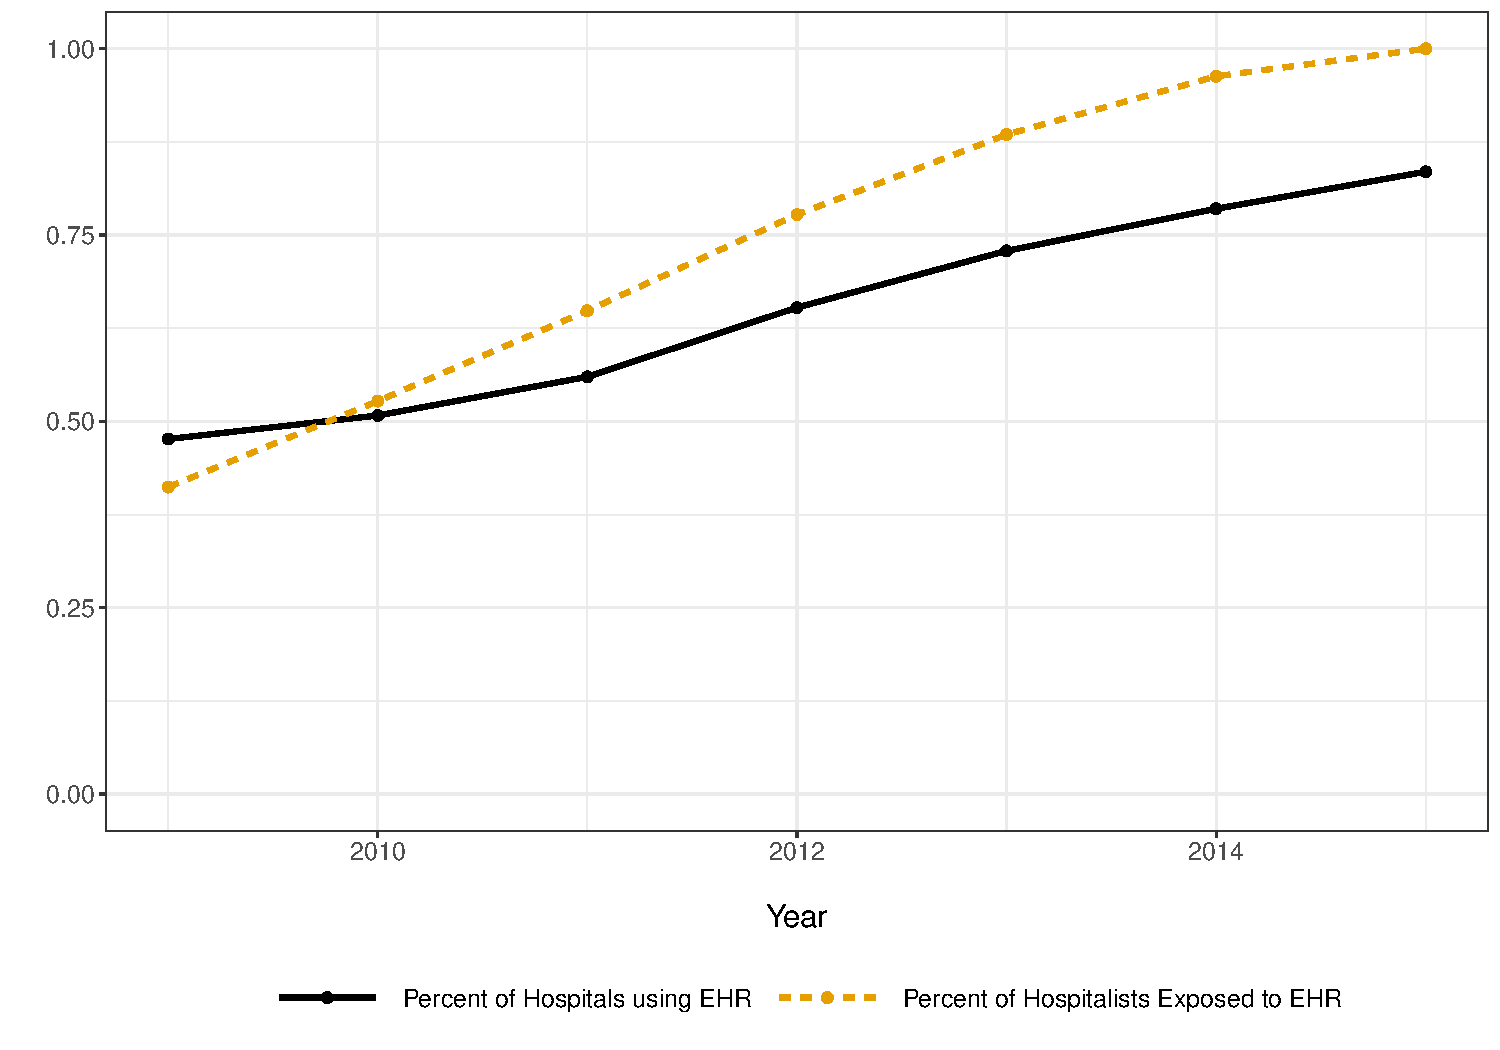
\includegraphics[scale=.6]{Objects/sum_stats_year.pdf}
    \label{fig:treatmentgraph}
\end{figure}


\section{Empirical Strategy}

In this setting, treatment effects likely vary across physicians who are exposed in different years since the underlying hospitals who implement likely vary. Therefore, to avoid negative weighting issues that arise in a two way fixed effects specification, I utilize \citeauthor{callaway2021difference} (\citeyear{callaway2021difference}) to estimate average group time treatment effects (ATT(g,t)). There are several assumptions I make to identify ATT(g,t).

\subsection{Anticipation}

 The first assumption necessary for identification is that anticipation either does not exist or is well understood. The estimator can takes anticipation into account as long as the duration is well understood and the same for all units. Anticipation plays into EHR implementation in an interesting way. Since the technology has different vendors and varies in capabilities, anticipation may be a concern if physicians learn that the system will be implemented and then do not actually use it until years later. Generally, even a complex EHR system can be completely set up within a year, and most systems take 6 to 9 months (\cite{uzialko_2021}). Therefore, in my main specification I assume there is no anticipation in physicians. In Appendix (\textcolor{red}{section}), I show results under the assumption of a one year anticipation period. 

\subsection{Parallel Trends with Not-yet-treated}

\subsection{No Treatment Reversal and Overlap}




\section{Retirement}

It is not uncommon in developed countries for workers to plan for formal retirement well in advance. An exogenous shock to a worker is not expected to change retirement age because of the large sum of money necessary to formally leave the labor force. However, physicians typically make this decision differently than most other workers. Most physicians plan to retire at age 60, but do not actually retire until age 69 (\cite{collier2017challenges}). When it comes time to retire, many physicians hesitate to abandon patients they have seen over the course of their career. This decision to delay retirement is not financial, but altruistic. Thus, retiring may be in a physician's choice set years before the realized decision to leave the labor force. Further, formal retirement is not the only way to stop seeing patients. There are opportunities for physicians of any age to switch careers towards more administrative roles such as teaching, consulting, hospital management, etc. While young physicians are probably not retiring in the traditional sense, either old or young physicians could be career switching. The term "retirement" for the purpose of this paper remains agnostic about what the physician does after they stop seeing patients in a clinical setting. 

An exogenous shock to work setting, such as EHR implementation in place of work, may cause an earlier exit than would have occurred without the shock. Medical articles suggest through interaction with physicians that the implementation of EHRs led to retirement in older physicians. \textcolor{red}{cite articles}. The first aim of this section is to test that hypothesis.. 

\subsection{Effect of EHR Exposure on Retirement Decision: Event Study Results}

Figure \ref{fig:retirefirst} shows the aggregated group time treatment effects of being exposed to an EHR in any hospital. The top graph suggests that for any physician, being exposed to an EHR leads to an almost .0025 ppt increase in the likelihood of retiring in both the first and second year after after implementation. Relative to the sample mean, this is an increase of approximately 1\%. We can examine how this result differs when considering different age groups of physician. These results are shown in the bottom panels of Figure \ref{fig:retirefirst}, and suggest that old physicians are driving the result in the first year after EHR exposure. That is, a physician who is at least 60 years old is .005 ppts more likely to retire after being exposed to an EHR, a .25\% increase relative to the mean. The results for physicians less than 60 reveals something interesting, that the younger physicians are driving the results in the second year after exposure. If young physicians are choosing to leave clinical settings, this result is intuitive since career switching may take more time to prepare for than formal retirement.    




\begin{figure}[ht]
\caption{Event Study Graphs: Retirement}
\vspace{2mm}
\centering
\hspace{20mm}
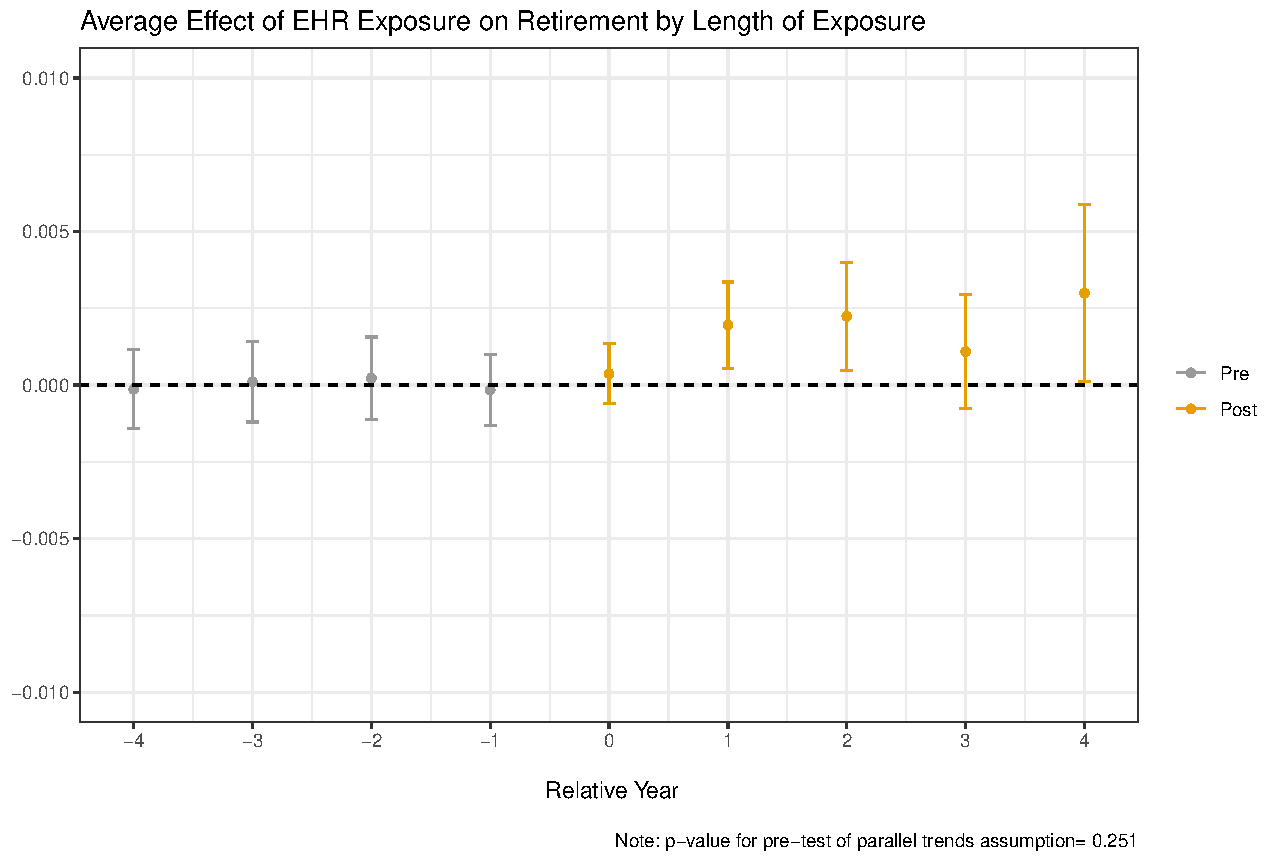
\includegraphics[scale=.4]{Objects/CS_retire_allEHR.pdf}
\vspace{3mm}
\newline
        \fbox{\begin{minipage}[b]{0.47\linewidth}
            \centering
            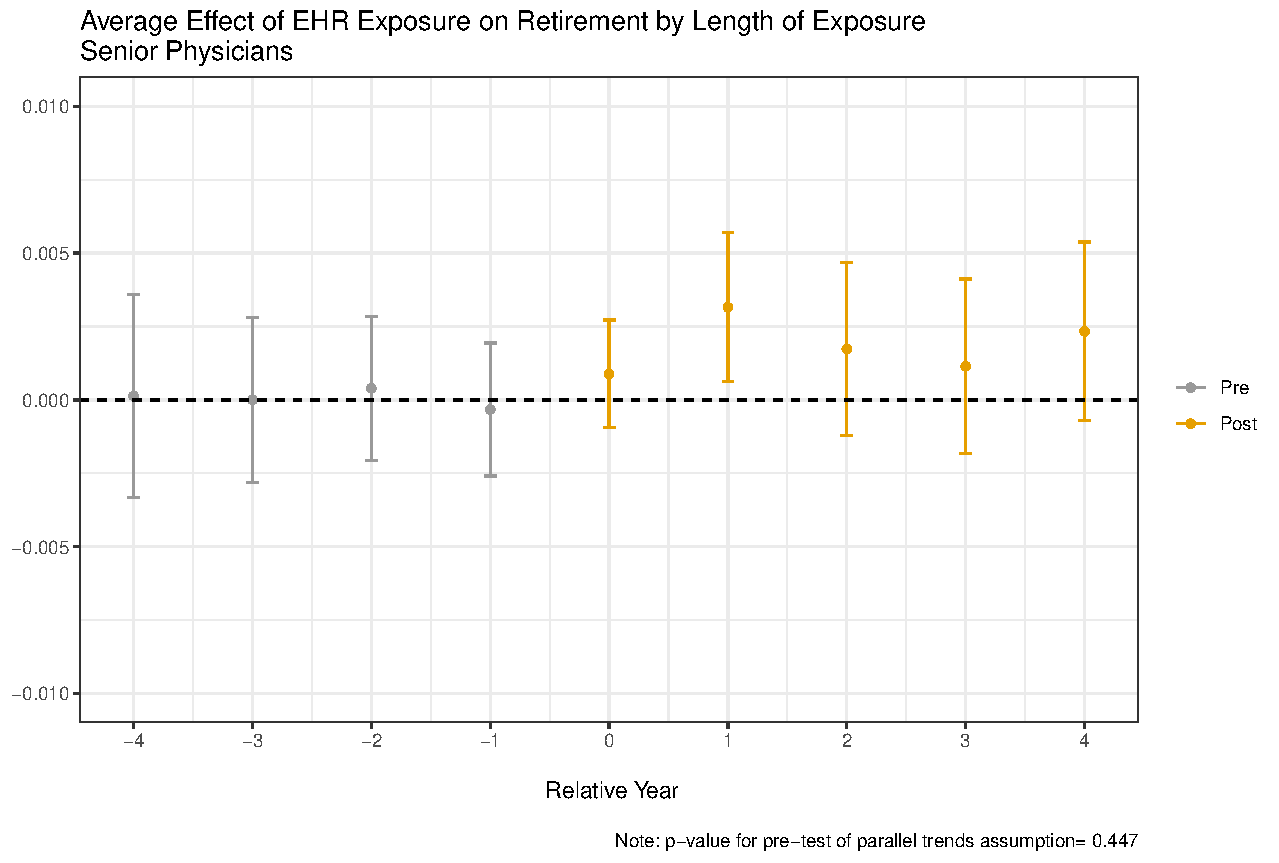
\includegraphics[width=\textwidth]{Objects/CS_retireold_allEHR.pdf}
        \end{minipage}}
        \hspace{0.1cm}
        \fbox{\begin{minipage}[b]{0.47\linewidth}
            \centering
            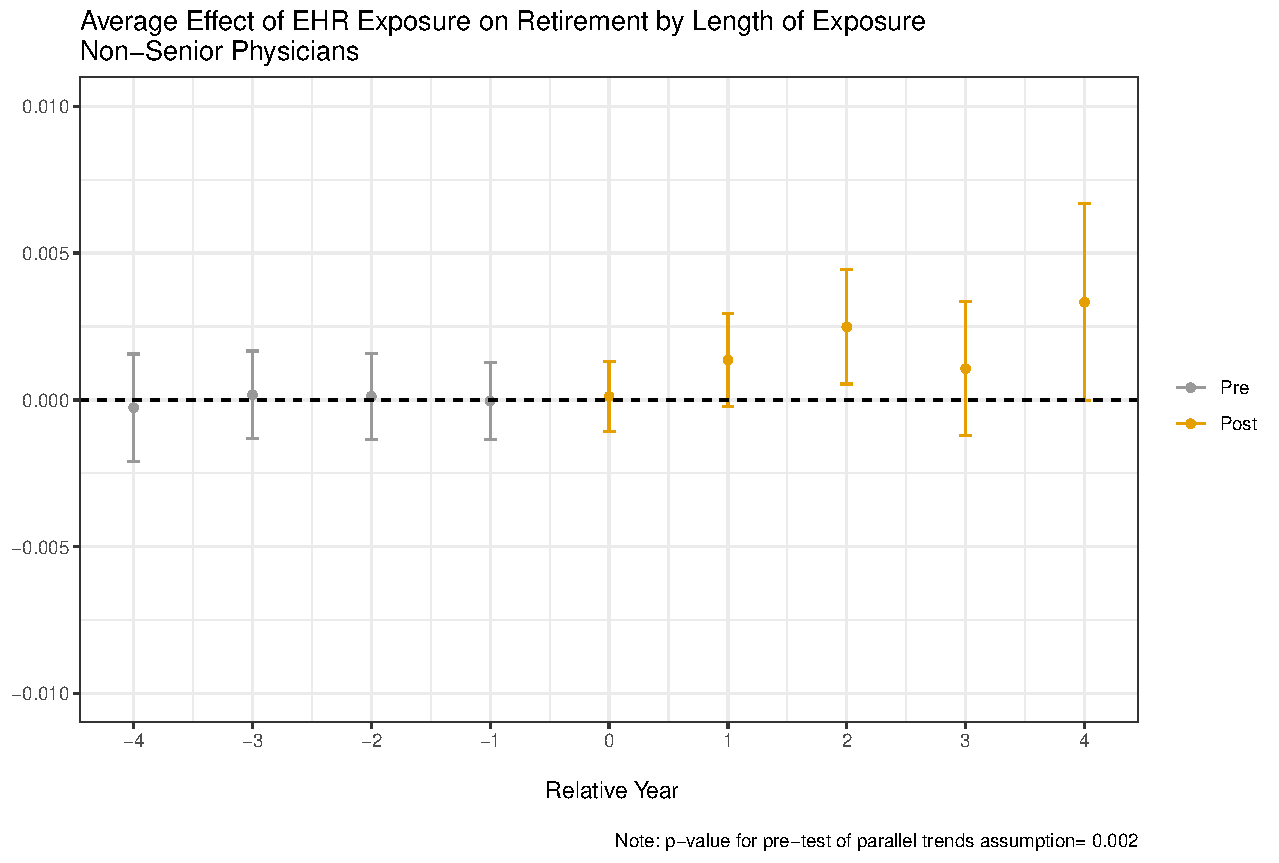
\includegraphics[width=\textwidth]{Objects/CS_retireyoung_allEHR.pdf}
        \end{minipage}}
        \label{fig:retirefirst}
\end{figure}



\subsection{Pre-Retirement Claim Counts}

If physicians are retiring because of EHRs, this may lead to the question of whether the physician is choosing to retire or the hospital is forcing older physicians out as they make major changes. To address this, I utilize claim counts in years prior to retirement. Some studies suggest that physicians may significantly reduce work or work part-time in preparation for formal retirement (\cite{hedden2017patterns}, \cite{acp_2017}). If there is evidence of physicians reducing workload prior to retirement, that is indicative of physicians choosing to retire as a result of EHR exposure. Thus, I seek to answer the question do physicians of retirement age reduce patients seen due to EHRs relative to other populations? Did physicians who eventually retire in the sample reduce patients seen prior to retirement? 




\section{Work Setting}

\newpage

\section{Physician Productivity}

An important aspect in the implementation of EHRs is whether or not they increase productivity in users. Productivity, in this case, has two key determinants: the choice of physicians to learn and utilize the technology, and the realized quality/innovation of electronic health records themselves. Regarding the first determinant, I will assume that when a physician continues to work in an electronic record utilizing-hospital, they utilize the electronic health record system fully. That is, there are no physicians who stay actively working in a hospital but choose not to partake in the electronic health record used by the hospital. To understand the second determinant, the value added of electronic health records themselves, the sample of physicians is limited to those who have patients in hospitals even after EHR exposure. 

It is reasonable to believe that physicians are fully utilizing the EHRs in the hospital they work in, since by 2015 electronic health records were widely implemented and considered unavoidable. An objection to this assumption may be that older physicians stay in a hospital, but the hospital hires a data assistant to do technology work for the physician. In this case, the productivity gain could be from having the data assistant instead of EHR use. I investigate this below.

\subsection{Data Assistants}

One concern with this measure of productivity is that an increase in the number of patients seen by a physician could be caused by an outside factor that is also correlated with EHR adoption in hospitals. A logical outside factor could be the existence of employees with the purpose of utilizing electronic health records on a physician's behalf. Employees of this type are assigned a medical tax ID when working in hospitals; they have the following titles: Coding Specialist (Hospital Based), Health Information Technologist and Registered Record Administrator. I will refer to any employee in these categories as a data assistant. 

Using NPPES data on all NPIs and their tax information, I analyze the existence of data assistants in hospitals. Figure \textcolor{red}{number} is a frequency plot of the year of activation for every tax code that falls in the categories listed above. The total number of these registered employees is 875. The first data assistants ever registered were in 2005, when electronic medical records were being implemented. From 2005 to 2013, more 15-60 more employees were registered each year. The graph is clearly skewed towards later years, where a significant increase in the number of new data assistants occured in 2014. If hiring data assistants were directly correlated with both EHR implementation and physician frustration, one would expect the increase to occur from 2011-2012, when a majority of physicians were first exposed to EHRs. 


\vspace{5mm}
\begin{figure}[ht]
\caption{Frequency of Data Assistant Enumeration by Year}

    \label{fig:dataassistant_histogram}
\end{figure}

The total number of registered data assistants may not equal the true number of people doing a data assistant job in hospitals. However, under the assumption that the number of registered data assistants is proportional to the number of actual data assistants, the claim of no correlation still holds. 


\subsection{Event Study Results}






\subsection{Relaxing Exogeneity of Implementation}


\textcolor{red}{I need to put somewhere that i dropped 2015 for this analysis since it cut off at a different point than the other years}

\renewcommand*{\bibfont}{\footnotesize}

\printbibliography

\newpage

\appendix

\section{}








\end{document}